\documentclass[dvipdfmx,autodetect-engine,titlepage]{jsarticle}
\usepackage[dvipdfm]{graphicx}
\usepackage{ascmac}
\usepackage{fancybox}
\usepackage{listings}
\usepackage{plistings}
\usepackage{itembkbx}
\usepackage{amsmath}
\usepackage{svg}
\usepackage{url}
\usepackage{graphics}
\usepackage{listings,jvlisting}
\usepackage{scalefnt}

\textheight=23cm
\renewcommand{\figurename}{図}
\renewcommand{\tablename}{表}
\newenvironment{code}
{\vspace{0.5zw}\VerbatimEnvironment  
\begin{screen} 
\baselineskip=1.0\normalbaselineskip
 \begin{Verbatim}}
{\end{Verbatim}
\baselineskip=\normalbaselineskip
 \end{screen}\vspace{0.5zw}} 

\title{情報理工学部 SNコース 2回\\
セキュリティ・ネットワーク学実験2\\
課題7レポート}
\author{2600200443-6\\Yamashita Kyohei\\山下 恭平}
\date{November 1 2021}

\begin{document}

\maketitle

\section{概要}
 BLE(Bluetooth Low Energy)を用いてRaspberry Piとアンドロイドスマートフォン
 間で通信を行い、独自のIoTデバイスを作成する。

\section{外部仕様}

 \subsection{開発対象の使い方に関する説明}
  Raspberry Piにはセンサとして超音波レンジャーが接続されており、測定された距離によって
  アクチュエータである、ディスプレイの色が変更されるようになっている。また、スマート
  フォンには、センサが測定した値がグラフとして表示されるようになっている。

 \begin{figure}[h]
    \centering
    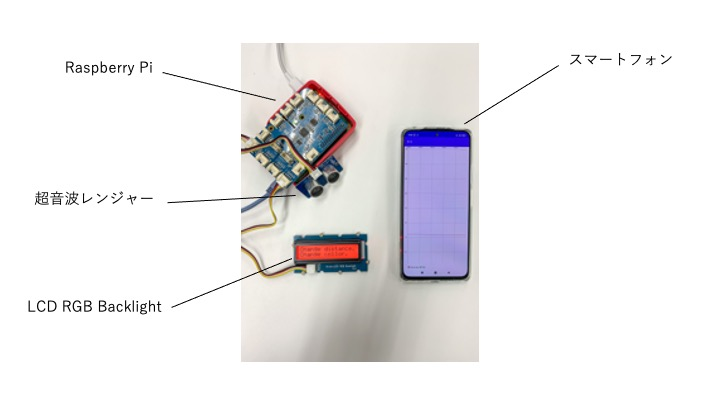
\includegraphics[scale=0.5]{pic1.jpg}
    \caption{開発したデバイス}
  \end{figure}


 \subsection{開発対象を構成するハードウェアと、その主な仕様}
 Raspberry PiにはGrove Starter Kit のシールドを利用し、各センサやアクチュエータ
 を接続した。また、Raspberry Piはセンサから情報の取得、アクチュエータの制御など、デバイス
 の主要部分ほとんどを担っている。超音波レンジャーは超音波により距離を測定しており、精度は
 1cm単位で測定可能である。LCD RGB Backlightは背景色を赤緑青それぞれを256段階で調節
 可能なディスプレイであり、任意の色、文字を表示することができる。スマートフォンはセントラル
 として使用しており、測定した値をもとにディスプレイの色を決定する演算をおこなっている。以下の
 表に全てのハードウェアをまとめる。\\\\

 \begin{table}[h]
    \caption{ハードウェア一覧}
    \begin{tabular}{cll}
    \hline
    機器一覧              & \multicolumn{1}{c}{} & \multicolumn{1}{c}{仕様/情報}             \\ \hline\hline
    Raspberry Pi      &                      & センサ、アクチュエータを接続しそれらの制御を行う。ペリフェラルとして使用。 \\ \hline
    超音波レンジャー          &                      & 超音波を送り、物体からのエコーを受信し、距離を測定。            \\ \hline
    LCD RGB Backlight &                      & RGBバックライトを搭載したディスプレイ。                 \\ \hline
    スマートフォン           &                      & Androidスマートフォン。セントラルとして使用。            \\ \hline
    \end{tabular}
    \end{table}

 
 \subsection{ハードウェアやソフトウェアが担当する機能と、機能同士の関連}
 まず、超音波レンジャーから距離を測定し、その値をRaspberry Piで取得、Raspberry Pi
 からスマートフォンへ向けてデータを送信、スマートフォンから送られてきたデータをディスプレイ
 に出力まで、これらががRaspberry Piが担う役割である。スマートフォンは測定結果を受信したら
 それをグラフへ表示、その結果をもとに送信するデータの作成、データの送信を担う。以下の図は
 それらの構成をまとめたものである。

 \begin{figure}[h]
    \centering
    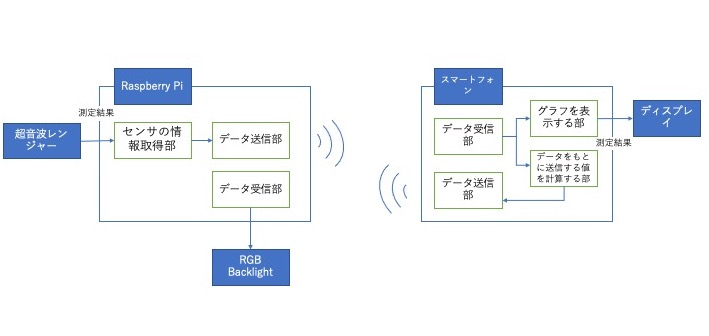
\includegraphics[scale=0.6]{pic2.jpg}
    \caption{機能構成図}
  \end{figure}

 
 \subsection{開発に用いたプログラミング言語と開発環境}
 今回の実験ではRaspberry Piの開発にJupyter Notebookを使用し、Pythonにてコーディングを
 行った。スマートフォンの開発にはAndroid Studioを使用しプログラミング言語としてJavaを
 使用した。以下の表は、開発環境をまとめたものである。
 \begin{table}[h]
    \centering
    \caption{まとめ表}
    \begin{tabular}{cll}
    \hline
    \multicolumn{3}{c}{開発環境}                             \\ \hline\hline
    OS            &  & macOS Monterey                    \\ \hline
    使用したアプリケーション  &  & Jupyter Notebook , Android Studio \\ \hline
    使用したプログラミング言語 &  & Python , Java                     \\ \hline
    \end{tabular}
    \end{table}

\section{内部仕様}

  \subsection{各ハードウェアが備えるソフトウェアの詳細な設計}
  Raspberry Pi側では、スマートフォンへデータを送信する関数notifyやアクチュエータの
  設定を行うsetText,setRGB、またセンサの制御としてranger,ultrasonicReadを使用した。\\
  スマートフォン側では、受信データと電波強度の両方を格納するための配列values[]を使用し、
  また、受信データを基に送信データを作成するDecideControlParameterや、これらの実行や
  送信データの設定などを行うonCharacteristicChangedなどを使用した。以下の表3,4は
  開発デバイスごとに主な設計を表にまとめたものである。
  \begin{table}[h]
    \centering
    \caption{Raspberry Piおよびセンサ、アクチュエータ}
    \begin{tabular}{clc}
    \hline
    関数名/クラス名/変数名                   &  & 説明                                      \\ \hline\hline
    Peripheral                 &  & BLE通信を管理するクラス、広告パケットの送信などに使用。           \\ \hline
    notify                     &  & セントラル(スマートフォン)へデータを送信する関数、センサの値を送信。     \\ \hline
    setText()                  &  & ディスプレイに表示する文字を設定。                       \\ \hline
    setRGB(int , int ,int)     &  & ディスプレイの色を設定。赤、青、緑の三色を0から255の256段階で調節可能。 \\ \hline
    ultrasonicRead(portnumber) &  & 指定したポート番号から超音波レンジャーの値を取得。int型の戻り値。      \\ \hline
    ranger                     &  & 超音波レンジャーを接続するポート番号を指定。int型。                  \\ \hline
    \end{tabular}
    \end{table}

    \begin{table}[h]
        \centering
        \small
        \caption{Java}
        \begin{tabular}{cll}
        \hline
        関数名/クラス名/変数名                 &  & \multicolumn{1}{c}{説明}                                       \\ \hline\hline
        values{[}{]}                 &  & values{[}0{]}:ペリフェラルから受信したデータを格納。int型。                       \\ \hline
                                     &  & values{[}1{]}:ペリフェラルから広告パケットを受信した時の電波強度を格納。int型。             \\ \hline
        DecideControlParameter(int ) &  & 引数(受信データ)を基に送信するデータを作成、int型の戻り値。                             \\ \hline
        onCharacteristicChanged      &  & values{[}1{]}へ電波強度を格納、DecideControlParameterの実行、送信データの設定を行う。 \\ \hline
        \end{tabular}
        \end{table}

  \subsection{各ハードウェアが備えるソフトウェアにおける処理の流れ}
  Raspberry Pi側では接続が確立したら、センサの値を取得、その値をスマートフォンへ送信、
  データを受信、受信データを基にディスプレイカラーを変更といった流れを無限ループで回し
  ている。スマートフォン側では、データを受信、データをグラフへ出力、送信するデータの作成
  、データの送信といった流れを同様に無縁ループで回すことで、双方での連続的な通信を確立している。
  以下は、それぞれのデバイスについてのフローチャートである。

  \begin{figure}[h]
    \centering
    \begin{minipage}[b]{0.45\linewidth}
    \begin{center}
      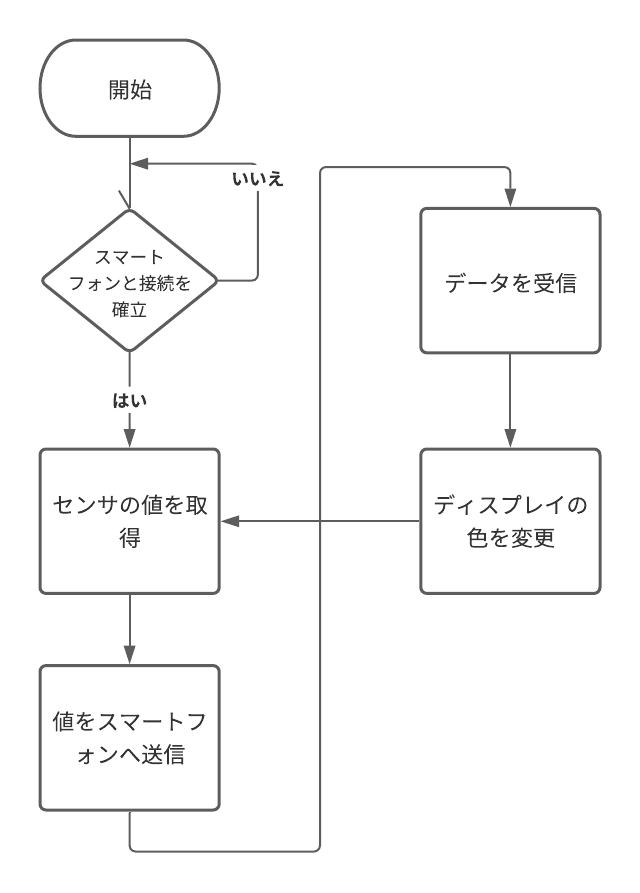
\includegraphics[keepaspectratio,scale=0.5]{フローチャート1.png}
      \end{center}
      \caption{Raspberry Pi}
    \end{minipage}
    \begin{minipage}[b]{0.45\linewidth}
    \begin{center}
      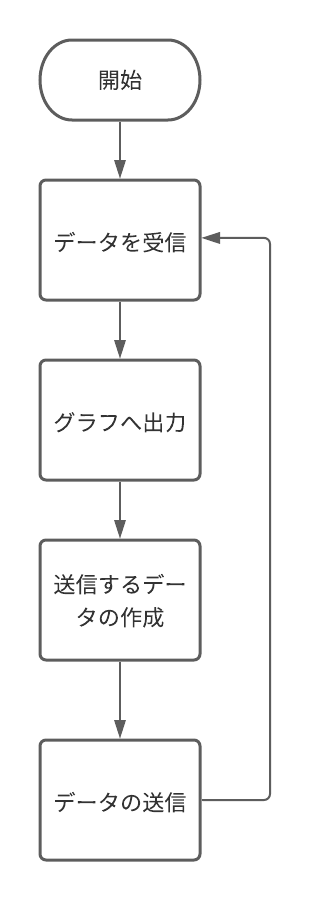
\includegraphics[keepaspectratio,scale=0.5]{フローチャート2.png}
      \end{center}
      \caption{スマートフォン}
    \end{minipage}
  \end{figure}


\section{実行例}
実験は、超音波レンジャーを固定し、箱を前に置き、この箱の距離を徐々に遠ざけていくことで
事件を行った。実験の結果距離が離れていくにつれて、ディスプレイの色はより緑いろへと近づき、
逆に距離が近い時は赤色を示した。実際の測定結果、ディスプレイの様子および実験の様子を以下の
図5,6,7に示す。

\begin{figure}[h]
    \centering
    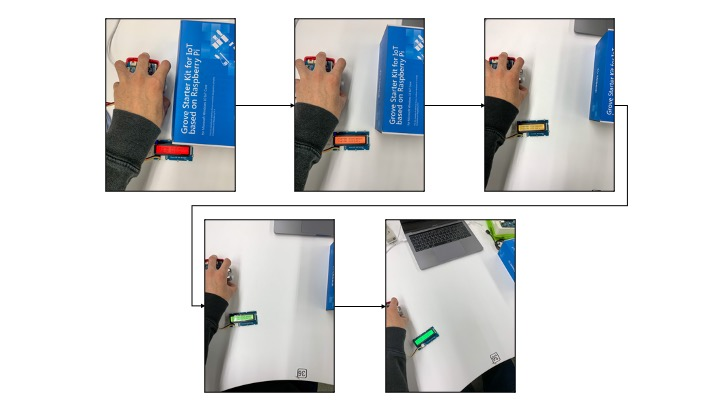
\includegraphics[scale=0.5]{実行例1.jpg}
    \caption{実行例1}
  \end{figure}

  \begin{figure}[h]
    \centering
    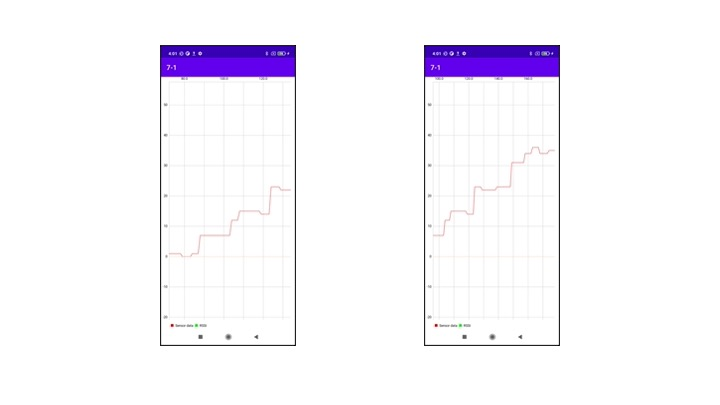
\includegraphics[scale=0.5]{実行例2.jpg}
    \caption{実行例2}
  \end{figure}

  \begin{figure}[h]
    \centering
    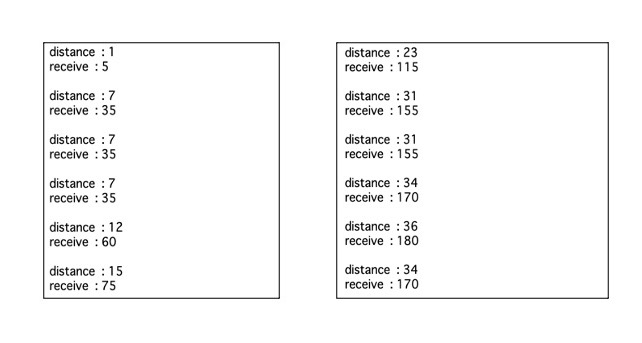
\includegraphics[scale=0.5]{実行例3.jpg}
    \caption{実行例3}
  \end{figure}



\section{ソースコード}
Raspberry Pi側では104行目で超音波レンジャーのポートを設定しており、116行目で
センサの値を取得、122行目でデータをスマートフォンへ送信し、128行目でスマートフォンから
データを受信、そして137行目でディスプレイの色を変更している。\\
スマートフォン側はDecideControlParameterにて、受信データを基に送信するデータを作成
している。

\lstset{
  basicstyle={\ttfamily},
  identifierstyle={\small},
  commentstyle={\smallitshape},
  keywordstyle={\small\bfseries},
  ndkeywordstyle={\small},
  stringstyle={\small\ttfamily},
  frame={tb},
  breaklines=true,
  columns=[l]{fullflexible},
  numbers=left,
  xrightmargin=0zw,
  xleftmargin=3zw,
  numberstyle={\scriptsize},
  stepnumber=1,
  numbersep=1zw,
  lineskip=-0.5ex
  }

  \begin{lstlisting}[caption=7-1.py,label=python]
from pybleno import *
from grovepi import *
from grove_rgb_lcd import *
import time

DEVICE_NAME = 'SecNet2_4436'
SERVICE_UUID = '19B10010-E8F2-537E-4F6C-D104768A1214'
WRITE_CHARACTERISTIC_UUID = '19B10011-E8F2-537E-4F6C-D104768A1214'
NOTIFY_CHARACTERISTIC_UUID = '19B10012-E8F2-537E-4F6C-D104768A1214'

class WriteCharacteristic(Characteristic):

    def __init__(self):
        Characteristic.__init__(self, {
            'uuid': WRITE_CHARACTERISTIC_UUID,
            'properties': ['write'],
            'value': None
        })

        self._value = str(0)
        self._updateValueCallback = None

    def onWriteRequest(self, data, offset, withoutResponse, callback):
        self._value = data.decode();
        callback(result=Characteristic.RESULT_SUCCESS)
       
        
class NotifyCharacteristic(Characteristic):

    def __init__(self):
        Characteristic.__init__(self, {
            'uuid': NOTIFY_CHARACTERISTIC_UUID,
            'properties': ['read', 'notify'],
            'value': None
        })

        self._value = str(0).encode()
        self._updateValueCallback = None

    def onSubscribe(self, maxValueSize, updateValueCallback):
        print('NotifyCharacteristic - onSubscribe')

        self._updateValueCallback = updateValueCallback

    def onUnsubscribe(self):
        print('NotifyCharacteristic - onUnsubscribe')

        self._updateValueCallback = None
        
        
class Peripheral():
    def __init__(self):
        self.bleno = Bleno()
        self.writeCharacteristic = WriteCharacteristic()
        self.notifyCharacteristic = NotifyCharacteristic()
        self.SERVICE_UUID = SERVICE_UUID

    def onStateChange(self, state):
        print('on -> stateChange: ' + state)

        if (state == 'poweredOn'):
            self.bleno.startAdvertising(name=DEVICE_NAME, service_uuids=[self.SERVICE_UUID])
        else:
            self.bleno.stopAdvertising()

    def onAdvertisingStart(self, error):
        print('on -> advertisingStart: ' + ('error ' + error if error else 'success'))

        if not error:
            self.bleno.setServices([
                BlenoPrimaryService({
                    'uuid': self.SERVICE_UUID,
                    'characteristics': [
                        self.writeCharacteristic,
                        self.notifyCharacteristic
                    ]
                })
            ])

    def advertise(self):
        self.bleno.on('stateChange', self.onStateChange)
        self.bleno.on('advertisingStart', self.onAdvertisingStart)
        self.bleno.start()

def notify(data, characteristic):
    if characteristic._updateValueCallback:
#        characteristic._value = str(data)
        characteristic._value = data

        notificationBytes = str(characteristic._value).encode()
        characteristic._updateValueCallback(data=notificationBytes)


def main():
    # Peripherarl用クラスの初期化
    peripheral = Peripheral()
    # 広告パケットの送信開始
    peripheral.advertise()
    # Write/Notify通信用のCharacteristicを取得
    writeCharacteristic = peripheral.writeCharacteristic
    notifyCharacteristic = peripheral.notifyCharacteristic
    
    ranger = 4
    pinMode(ranger,"INPUT")

    # Centralと接続し、データ通信の準備が整うまで待つ
    while True:
        if notifyCharacteristic._updateValueCallback:
            break

    setText("Change distance.\nChange collor.")
    
    # Centralとの通信を繰り返し実行
    while True:
        
        sensor_value = ultrasonicRead(ranger)
        
        # 送信するデータ(文字列)を確認
        print('distance  : ' + str(sensor_value))
        
        # データ(文字列)をCentralへ送信
        notify(data=str(sensor_value), characteristic=notifyCharacteristic)
        
            
        time.sleep(0.5) # 500ミリ秒待機
        
        # データ(文字列)をCentralから受信
        recv_value = writeCharacteristic._value

        
        # 受信したデータ(文字列)を確認
        print('receive  : ' + recv_value )
        
        print('')
        
        
        setRGB(255 - int(recv_value),int(recv_value),0)
        
        
        time.sleep(2) # 500ミリ秒待機
        
if __name__ == '__main__':
    main()

  \end{lstlisting}


  \begin{lstlisting}[caption=Java.py,label=Java]
    package com.example.a7_1;

import androidx.appcompat.app.AppCompatActivity;

import android.os.Bundle;

import androidx.core.app.ActivityCompat;

import android.Manifest;
import android.bluetooth.BluetoothAdapter;
import android.bluetooth.BluetoothGatt;
import android.bluetooth.BluetoothGattCallback;
import android.bluetooth.BluetoothGattCharacteristic;
import android.bluetooth.BluetoothGattDescriptor;
import android.bluetooth.BluetoothGattService;
import android.bluetooth.BluetoothManager;
import android.bluetooth.BluetoothProfile;
import android.bluetooth.le.BluetoothLeScanner;
import android.bluetooth.le.ScanCallback;
import android.bluetooth.le.ScanResult;
import android.content.Context;
import android.content.pm.PackageManager;
import android.graphics.Color;
import android.util.Log;
import android.view.WindowManager;

import com.github.mikephil.charting.charts.LineChart;
import com.github.mikephil.charting.components.AxisBase;
import com.github.mikephil.charting.components.XAxis;
import com.github.mikephil.charting.components.YAxis;
import com.github.mikephil.charting.data.Entry;
import com.github.mikephil.charting.data.LineData;
import com.github.mikephil.charting.data.LineDataSet;
import com.github.mikephil.charting.formatter.IAxisValueFormatter;
import com.github.mikephil.charting.utils.Transformer;
import com.github.mikephil.charting.utils.ViewPortHandler;

import java.util.UUID;

public class MainActivity extends AppCompatActivity {
    private LineChart mLineChart;

    // 接続対象となるペリフェラルの名前(XXXXは学籍番号の下4桁)
    private static final String PERIPHERAL_NAME = "SecNet2_4436";

    // 接続対象となるサービスのUUID.
    private static final String SERVICE_UUID = "19B10010-E8F2-537E-4F6C-D104768A1214";

    // 接続対象となるキャラクタリスティックのUUID.
    private static final String CHAR_WRITE_UUID = "19B10011-E8F2-537E-4F6C-D104768A1214";
    private static final String CHAR_NOTIFY_UUID = "19B10012-E8F2-537E-4F6C-D104768A1214";

    // キャラクタリスティック設定UUID(固定値).
    private static final String CHARACTERISTIC_CONFIG_UUID = "00002902-0000-1000-8000-00805f9b34fb";

    // ペリフェラルと接続しない: 0, ペリフェラルと接続する: 1
    private int flag_connect = 1;

    // グラフ表示用の変数
    private int num;
    private float[] values;
    private String[] labels; // データのラベルを格納する配列
    private int[] colors; // グラフにプロットする点の色を格納する配列
    private float max, min;

    // 値をプロットするx座標
    private float count = 0;

    // BLEで利用するクラス群
    private BluetoothManager mBleManager;
    private BluetoothAdapter mBleAdapter;
    private BluetoothLeScanner mBleScanner;
    private BluetoothGatt mBleGatt;
    private BluetoothGattCharacteristic notifyCharacteristic, writeCharacteristic;

    @Override
    protected void onCreate(Bundle savedInstanceState) {
        super.onCreate(savedInstanceState);
        setContentView(R.layout.activity_main);

        // アプリ実行中はスリープしない
        getWindow().addFlags(WindowManager.LayoutParams.FLAG_KEEP_SCREEN_ON);

        num = 2;
        values = new float[num];
        labels = new String[num];
        colors = new int[num];

        for(int i=0; i<num; i++){
            values[i] = 0;
        }

        labels[0] = "Sensor data";
        labels[1] = "RSSI";


        colors[0] = Color.rgb(0xFF, 0x00, 0x00); // 赤
        colors[1] = Color.rgb(0x00, 0xFF, 0x00); // 緑
        //       colors[2] = Color.rgb(0x00, 0x00, 0xFF); // 青

        max = 120;
        min = -50;

        // グラフViewを初期化する
        initChart();

        // Bluetoothの使用準備.
        mBleManager = (BluetoothManager) getSystemService(Context.BLUETOOTH_SERVICE);
        mBleAdapter = mBleManager.getAdapter();

        // 一定間隔でグラフをアップデートする
        new Thread(new Runnable() {
            @Override
            public void run() {
                while (true) {
                    updateGraph();
                    try {
                        Thread.sleep(500);
                    } catch (Exception e) {
                        Log.e("Test", "例外出力", e);
                    }
                }
            }
        }).start();
    }

    @Override
    protected void onResume() {
        super.onResume();

        // *************************************************** //
        // Bluetooth関連の処理                                  //
        // *************************************************** //

        // 位置情報の利用許可を利用者に求める (BLEも位置情報として利用できるため,許可が必要)
        if (ActivityCompat.checkSelfPermission(this, Manifest.permission.ACCESS_FINE_LOCATION) != PackageManager.PERMISSION_GRANTED) {
            ActivityCompat.requestPermissions(this, new String[]{Manifest.permission.ACCESS_FINE_LOCATION}, 1);

            return;
        }

        // BLEが使用可能なら、通信相手をスキャン
        if ((mBleAdapter != null) || (mBleAdapter.isEnabled())) {
            mBleScanner = mBleAdapter.getBluetoothLeScanner();
            mBleScanner.startScan(scanCallback);
        }
    }

    private int DecideControlParameter(int input){
        int output;

        output = 5 * input;

        return output;
    }

    private final BluetoothGattCallback mGattCallback = new BluetoothGattCallback() {
        @Override
        public void onConnectionStateChange(BluetoothGatt gatt, int status, int newState)
        {
            // 接続状況が変化したら実行.
            if (newState == BluetoothProfile.STATE_CONNECTED) {
                // 接続に成功したらサービスを検索する.
                gatt.discoverServices();
            } else if (newState == BluetoothProfile.STATE_DISCONNECTED) {
                // 接続が切れたらGATTを空にする.
                if (mBleGatt != null)
                {
                    mBleGatt.close();
                    mBleGatt = null;
                }
            }
        }

        @Override
        public void onServicesDiscovered(BluetoothGatt gatt, int status)
        {
            // Serviceが見つかったら実行.
            if (status == BluetoothGatt.GATT_SUCCESS) {
                // UUIDが同じかどうかを確認する.
                BluetoothGattService service = gatt.getService(UUID.fromString(SERVICE_UUID));
                if (service != null)
                {
                    // 指定したUUIDを持つCharacteristicを確認する.
                    notifyCharacteristic = service.getCharacteristic(UUID.fromString(CHAR_NOTIFY_UUID));
                    writeCharacteristic = service.getCharacteristic(UUID.fromString(CHAR_WRITE_UUID));

                    if (notifyCharacteristic != null) {

                        // Service, CharacteristicのUUIDが同じならBluetoothGattを更新する.
                        mBleGatt = gatt;

                        // キャラクタリスティックが見つかったら、Notificationをリクエスト.
                        boolean registered = mBleGatt.setCharacteristicNotification(notifyCharacteristic, true);

                        Log.v("BLE", "Notification beginning");
                        // Characteristic の Notificationを有効化する.
                        BluetoothGattDescriptor descriptor = notifyCharacteristic.getDescriptor(
                                UUID.fromString(CHARACTERISTIC_CONFIG_UUID));

                        descriptor.setValue(BluetoothGattDescriptor.ENABLE_NOTIFICATION_VALUE);
                        mBleGatt.writeDescriptor(descriptor);
                    }
                }
            }
        }

        @Override
        public void onCharacteristicChanged(BluetoothGatt gatt, BluetoothGattCharacteristic characteristic)
        {
            byte[] recvValue;
            byte[] sendValue;
            final String text;
            int input, output;

            // キャラクタリスティックのUUIDをチェック(getUuidの結果が全て小文字で帰ってくるのでUpperCaseに変換)
            if (CHAR_NOTIFY_UUID.equals(characteristic.getUuid().toString().toUpperCase()))
            {
                recvValue = characteristic.getValue();
                input = Integer.parseInt(new String(recvValue)); // 受信したデータを整数値に変換
                Log.v("BLE", "Received : " + input);

                values[0] = input;

                // ペリフェラルから受信したデータを元に、ペリフェラルへ送信するデータを算出
                output = DecideControlParameter(input);

                sendValue = String.valueOf(output).getBytes(); // 送信するデータを文字列に変換

                writeCharacteristic.setValue(sendValue);
                mBleGatt.writeCharacteristic(writeCharacteristic);
                Log.v("BLE", "Sent : " + output);

            }
        }
    };

    private ScanCallback scanCallback = new ScanCallback(){
        @Override
        public void onScanResult(int callbackType, ScanResult result) {
            super.onScanResult(callbackType, result);

            // 発見したペリフェラルが接続対象と一致する場合には、Rssiを取得
            if((result.getDevice().getName() != null) && (result.getDevice().getName().equals(PERIPHERAL_NAME))){
                values[1] = result.getRssi();

                String text = "Found: " + result.getDevice().getName() + ", " + values[1];
                Log.d("blelog", text);

                if(flag_connect == 1){
                    result.getDevice().connectGatt(getApplicationContext(), false, mGattCallback);
                }
            }
        }

        @Override
        public void onScanFailed(int intErrorCode) {
            super.onScanFailed(intErrorCode);
        }
    };

    /** グラフViewの初期化 **/

    private void initChart() {
        // 線グラフView
        mLineChart = (LineChart) findViewById(R.id.chart_DynamicMultiLineGraph);

        // グラフ説明テキストを表示するか
        mLineChart.getDescription().setEnabled(true);
        // グラフ説明テキストのテキスト設定
        mLineChart.getDescription().setText("Line Chart of Sensor Data");
        // グラフ説明テキストの文字色設定
        mLineChart.getDescription().setTextColor(Color.BLACK);
        // グラフ説明テキストの文字サイズ設定
        mLineChart.getDescription().setTextSize(10f);
        // グラフ説明テキストの表示位置設定
        mLineChart.getDescription().setPosition(0, 0);

        // グラフへのタッチジェスチャーを有効にするか
        mLineChart.setTouchEnabled(true);

        // グラフのスケーリングを有効にするか
        mLineChart.setScaleEnabled(true);

        // グラフのドラッギングを有効にするか
        mLineChart.setDragEnabled(true);

        // グラフのピンチ/ズームを有効にするか
        mLineChart.setPinchZoom(true);

        // グラフの背景色設定
        mLineChart.setBackgroundColor(Color.WHITE);

        // 空のデータをセットする
        mLineChart.setData(new LineData());

        // Y軸(左)の設定
        // Y軸(左)の取得
        YAxis leftYAxis = mLineChart.getAxisLeft();
        // Y軸(左)の最大値設定
        leftYAxis.setAxisMaximum(max);
        // Y軸(左)の最小値設定
        leftYAxis.setAxisMinimum(min);

        // Y軸(右)の設定
        // Y軸(右)は表示しない
        mLineChart.getAxisRight().setEnabled(false);

        // X軸の設定
        XAxis xAxis = mLineChart.getXAxis();
        // X軸の値表示設定
        xAxis.setValueFormatter(new IAxisValueFormatter() {
            @Override
            public String getFormattedValue(float value, AxisBase axis) {
                if(value >= 10) {
                    // データ20個ごとに目盛りに文字を表示
                    if (((int) value % 20) == 0) {
                        return Float.toString(value);
                    }
                }
                // nullを返すと落ちるので、値を書かない場合は空文字を返す
                return "";
            }
        });
    }

    private void updateGraph() {
        // 線の情報を取得
        LineData lineData = mLineChart.getData();
        if(lineData == null) {
            return;
        }

        LineDataSet[] lineDataSet = new LineDataSet[num];

        for(int i = 0; i<num; i++){
            // i番目の線を取得
            lineDataSet[i] = (LineDataSet) lineData.getDataSetByIndex(i);
            // i番目の線が初期化されていない場合は初期化する
            if( lineDataSet[i] == null) {
                // LineDataSetオブジェクト生成
                lineDataSet[i] = new LineDataSet(null, labels[i]);
                // 線の色設定
                lineDataSet[i].setColor(colors[i]);
                // 線にプロット値の点を描画しない
                lineDataSet[i].setDrawCircles(false);
                // 線にプロット値の値テキストを描画しない
                lineDataSet[i].setDrawValues(false);
                // 線を追加
                lineData.addDataSet(lineDataSet[i]);
            }
            // i番目の線に値を追加
            lineData.addEntry(new Entry(count, values[i]), i);
        }

        // 値更新通知
        mLineChart.notifyDataSetChanged();

        // X軸に表示する最大のEntryの数を指定
        mLineChart.setVisibleXRangeMaximum(100);

        // オシロスコープのように古いデータを左に寄せていくように表示位置をずらす
        mLineChart.moveViewTo(count, getVisibleYCenterValue(mLineChart), YAxis.AxisDependency.LEFT);

        count++;
    }

    /**
     * 表示しているY座標の中心値を返す<br>
     *     基準のY座標は左
     * @param lineChart 対象のLineChart
     * @return 表示しているY座標の中心値
     */
    private float getVisibleYCenterValue(LineChart lineChart) {
        Transformer transformer = lineChart.getTransformer(YAxis.AxisDependency.LEFT);
        ViewPortHandler viewPortHandler = lineChart.getViewPortHandler();

        float highestVisibleY = (float) transformer.getValuesByTouchPoint(viewPortHandler.contentLeft(),
                viewPortHandler.contentTop()).y;
        float highestY = Math.min(lineChart.getAxisLeft().mAxisMaximum, highestVisibleY);

        float lowestVisibleY = (float) transformer.getValuesByTouchPoint(viewPortHandler.contentLeft(),
                viewPortHandler.contentBottom()).y;
        float lowestY = Math.max(lineChart.getAxisLeft().mAxisMinimum, lowestVisibleY);

        return highestY - (Math.abs(highestY - lowestY) / 2);
    }
}
  \end{lstlisting}

\section{センサネットワーク実験に対する感想}
センサやアクチュエータを初めて使用することができ、また、アプリの開発も同時に行うことが
できたので、非常に満足できる実験であった。



\end{document}

